This chapter briefly explores the state of art in space grade solar and battery cell technologies. \refSec{sec:StateOfTheArt:PastAndOngoingMissions} presents an overview of past and ongoing missions. The state of practice is briefly touched upon in \refSec{sec:StateOfTheArt:PlannedMissions} as a segue to the state of the art in \refSec{sec:StateOfTheArt:PhotovoltaicsAndEnergyStorage}.

\section{Past and Ongoing Missions}
\label{sec:StateOfTheArt:PastAndOngoingMissions}
% Image source:
% MER
% https://mars.nasa.gov/mer/

% All others:
% https://science.nasa.gov/toolkits/spacecraft-icons
The scope of this section is restricted to successful missions. At the time of writing this thesis, the \ac{NASA} remains the only organization to successfully land and operate a spacecraft on the Martian surface. Two types of missions are explored: landers and rovers. Descriptions of these missions are restricted to power generation and storage characteristics.

\subsection{Landers}
\label{sec:StateOfTheArt:PastAndOngoingMissions:Landers}

Successful landers are shown in Figure \ref{fig:past-mission-landers}. The Viking Program involved two space probes: Viking 1 and Viking 2. Each were composed of an orbiter and a lander, identified as \ac{VL1} and \ac{VL2} shown Figure \ref{fig:sub:past-mission-lander-viking}. The Phoenix lander, shown in Figure \ref{fig:sub:past-mission-lander-phoenix} was part of the Mars Scout Program. The ongoing InSight mission lander is part of the Discovery Program and is shown in Figure \ref{fig:sub:past-mission-lander-insight}.

\vspace{0.5cm}

\begin{figure}[h]
\captionsetup[subfigure]{justification=centering}
\vspace{-2ex}
	\centering
    %% setup sizes
    \setlength{\subfigureWidth}{0.48\textwidth}
    \setlength{\graphicsHeight}{31mm}
    %% kill hyper-link highlighting
    \hypersetup{hidelinks=true}%
    %% the figures
	\begin{subfigure}[t]{\subfigureWidth}
        \centering
		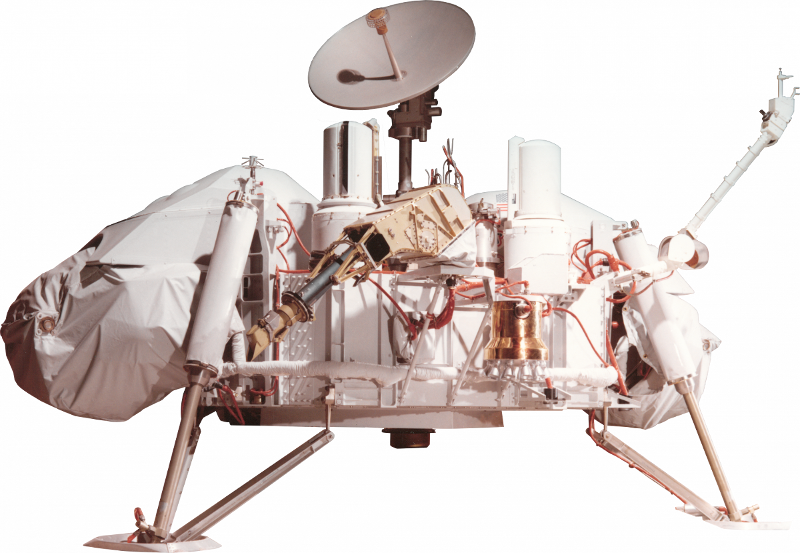
\includegraphics[height=\graphicsHeight]{sections/state-of-the-art/past-missions/images/lander-viking.png}
		\subcaption{Viking}
		\label{fig:sub:past-mission-lander-viking}
	\end{subfigure}\\[0.8ex]
%% 2nd row
	\begin{subfigure}[t]{\subfigureWidth}
        \centering
		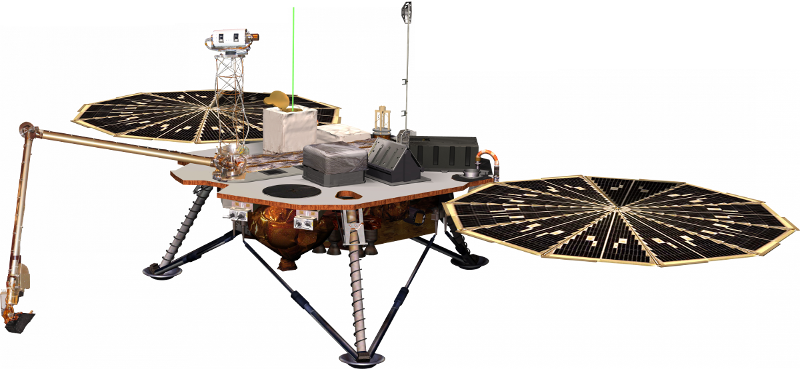
\includegraphics[height=\graphicsHeight]{sections/state-of-the-art/past-missions/images/lander-phoenix.png}
        \subcaption{Phoenix}
		\label{fig:sub:past-mission-lander-phoenix}
	\end{subfigure}\hspace*{0.5cm}
    \begin{subfigure}[t]{\subfigureWidth}
        \centering
		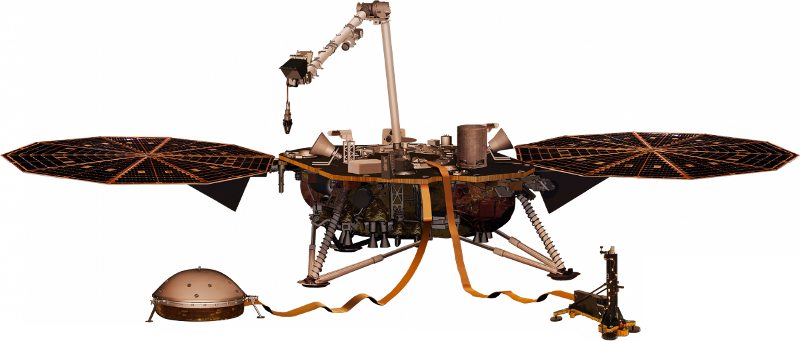
\includegraphics[height=\graphicsHeight]{sections/state-of-the-art/past-missions/images/lander-insight.png}
		\subcaption{InSight}
		\label{fig:sub:past-mission-lander-insight}
	\end{subfigure}
    \caption[Past and ongoing lander missions]
            {Past and ongoing lander missions.}
	\label{fig:past-mission-landers}
\vspace{-2ex}
\end{figure}

% Alternative layout of lander figures. All 3 subfigures in a single line.
\begin{comment}
\begin{figure}[h]
\captionsetup[subfigure]{justification=centering}
\vspace{-2ex}
	\centering
    %% setup sizes
    \setlength{\subfigureWidth}{0.32\textwidth}
    \setlength{\graphicsHeight}{21mm}
    %% kill hyper-link highlighting
    \hypersetup{hidelinks=true}%
    %% the figures
	\begin{subfigure}[t]{\subfigureWidth}
        \centering
		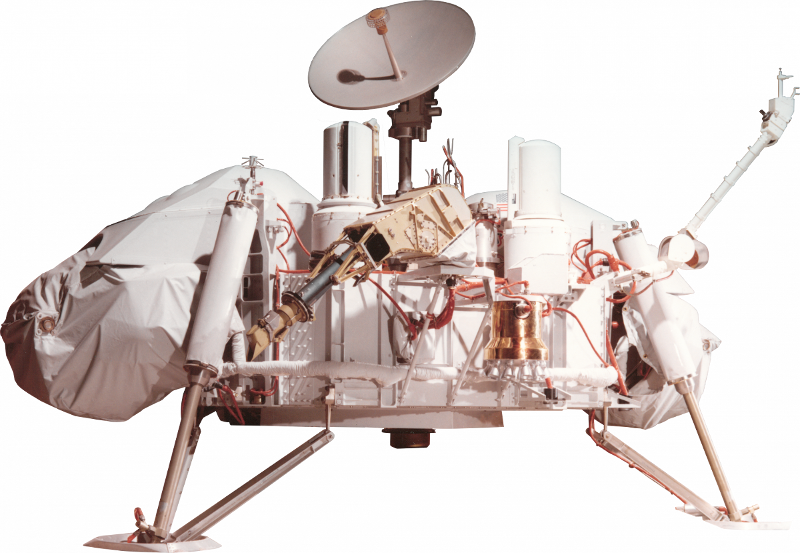
\includegraphics[height=\graphicsHeight]{sections/state-of-the-art/past-missions/images/lander-viking.png}
		\subcaption{Viking Lander}
		\label{fig:sub:past-mission-lander-viking}
	\end{subfigure}\hfill
	\begin{subfigure}[t]{\subfigureWidth}
        \centering
		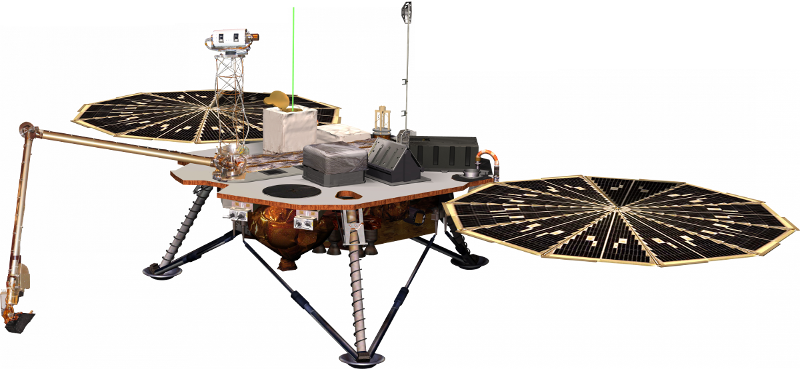
\includegraphics[height=\graphicsHeight]{sections/state-of-the-art/past-missions/images/lander-phoenix.png}
		\subcaption{Phoenix Lander}
		\label{fig:sub:past-mission-lander-phoenix}
	\end{subfigure}\hfill
    \begin{subfigure}[t]{\subfigureWidth}
        \centering
		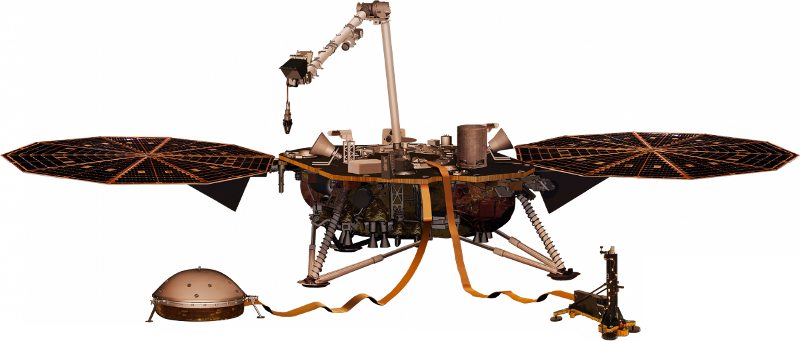
\includegraphics[height=\graphicsHeight]{sections/state-of-the-art/past-missions/images/lander-insight.png}
		\subcaption{InSight Lander}
		\label{fig:sub:past-mission-lander-insight}
	\end{subfigure}
	\caption[Past and ongoing lander missions]
            {Past and ongoing lander missions.}
	\label{fig:past-mission-landers}
\vspace{-2ex}
\end{figure}
\end{comment}

\subsubsection{Viking}

A single Viking Lander was powered by two \ac{RTG} units. Converting heat from decaying plutonium-236 resulted in a continuous nominal electrical power output of \SI{70}{\watt} at \SI{4.4}{\volt}. Four \SI{30}{\volt} nominal, 42-cell \ac{NiCd} batteries were mounted in pairs and charged by the \ac{RTG} units. The battery cells were \SI{8}{\ampere\hour} at \ac{EOL}. Recharge rates depended on available \ac{RTG} energy and varied from C/40 to C/6. Descrease in charge efficieny tied to temperature increase imposed a thermal constraint in which charging did not occur if the battery temperature was greater than \SI{21}{\degree} in order to prevent excessive battery temperatures during charging. Further power subsytem design details can be found in \citepower{Holmburg1980}.

\subsubsection{Phoenix}

The Phoenix Lander generated power from its two ATK ``UltraFlex'' \acp{SA} which covered a total surface area of \SI{4.2}{\meter\squared}. The \acp{SA} provided approximately \SI{22}{\watt/\kilo\gram} under Mars conditions \citepower{Badescu2009} \citeother{Linne2012}. Its round fan-fold design unfoled into two separate circular decagon panels. Two rechargeable \ac{Li-ion} \ac{NCO}-cell batteries were manufactured by Yardney and had a nameplate capacity of \SI{25}{\ampere\hour}. The battery cells were arranged in an 8s2p configuration, capacity voltage range was 50‒62 \si{\volt}, operating voltage range 24‒\SI{32.8}{\volt}, mass \SI{17.8}{\kilo\gram}, specific energy \SI{105}{\watt\hour/\kilo\gram}, and the operating temperature was from \SI{-20}{\celsius} to +\SI{30}{\celsius} \citepower{NASAEnergyStorage2017}.

\subsubsection{InSight}

The InSight Lander is based on heritage from the Phoenix mission and as such shares similar characteristics. It generates power from two \acp{SA} each measuring \SI{2.2}{\meter} in diameter. The \acp{SA} are  ATK ``UltraFlex'' ZTJ triple-junction solar cells made of \ac{InGaP}/\ac{InGaAs}/\ac{Ge}. The \ac{NCA}-cells rechargeable batteries were manufactured by Yardney and based on Phoenix's NCP‒25‒1 cell design. The two 8-cell in parallel (8s2p), \SI{28}{\volt}, \SI{30}{\ampere\hour} batteries can operate down to \SI{-35}{\celsius} \citepower{EaglePitcher}. As listed in \citepower{Smart2015}, the battery performance requirements for InSight are:

\begin{itemize}
  \item The battery shall support 709 sols of surface operations over a temperature range of \SI{-30}{\celsius} to +\SI{35}{\celsius}.
  \item Each 8-cell battery shall be able to support a \SI{5}{\ampere} charge rate over the entire allowable flight temperature range of \SI{-30}{\celsius} to +\SI{35}{\celsius}.
  \item Each 8-cell battery shall provide at least \SI{25}{\ampere\hour} at \SI{-25}{\celsius} \ac{BOL} over the voltage range of \SI{24}{\volt} to \SI{32.8}{\volt} using a C/5 rate (\SI{5}{\ampere}).
\end{itemize}

\clearpage
\subsection{Rovers}
\label{sec:StateOfTheArt:PastAndOngoingMissions:Rovers}

Successful rovers are shown in Figure \ref{fig:past-mission-rovers}. The Sojourner rover was the first rover to operate on the Martian surface and is shown in Figure \ref{fig:sub:past-mission-rover-sojourner}. The \ac{MER} mission consisted of twin rovers  Spirit and Opportunity shown in Figure \ref{fig:sub:past-mission-rovers-mer}. The ongoing \ac{MSL} Curiosity mission is part of the \ac{MEP} and shown in Figure \ref{fig:sub:past-mission-rovers-msl}.

\begin{figure}[h]
\captionsetup[subfigure]{justification=centering}
\vspace{-2ex}
	\centering
    %% setup sizes
    \setlength{\subfigureWidth}{0.45\textwidth}
    \setlength{\graphicsHeight}{35mm}
    %% kill hyper-link highlighting
    \hypersetup{hidelinks=true}%
    %% the figures
	\begin{subfigure}[t]{\subfigureWidth}
        \centering
        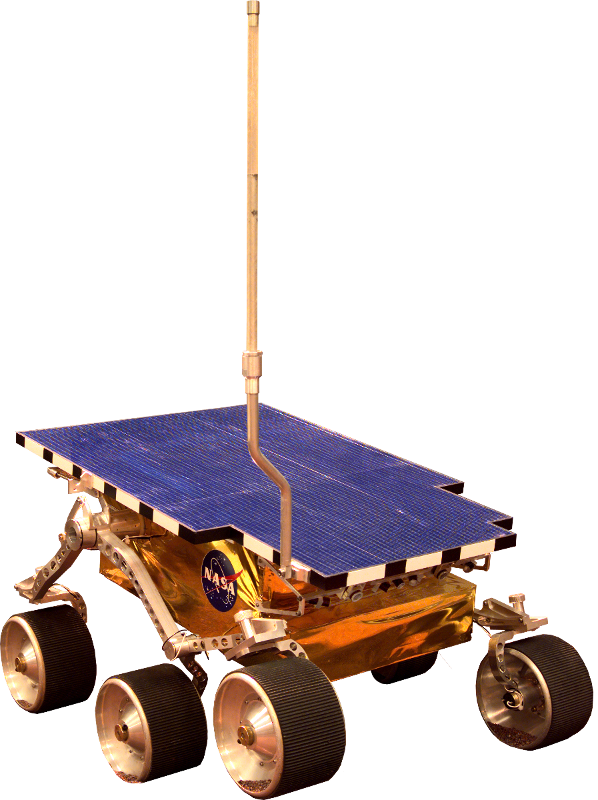
\includegraphics[height=\graphicsHeight]{sections/state-of-the-art/past-missions/images/rover-sojourner.png}
        \subcaption{Sojourner}
        \label{fig:sub:past-mission-rover-sojourner}
	\end{subfigure}\\[0.8ex]
%% 2nd row
	\begin{subfigure}[t]{\subfigureWidth}
        \centering
		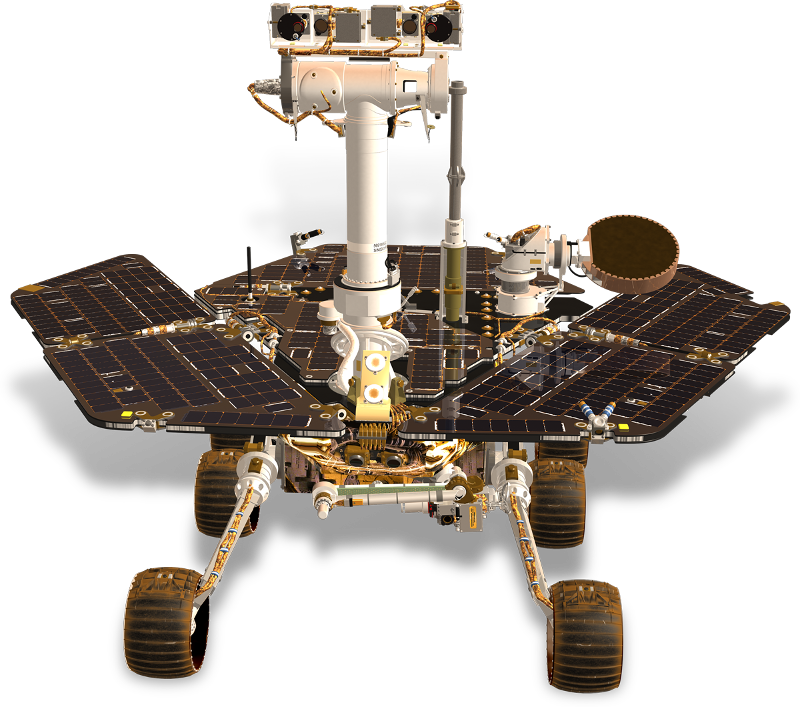
\includegraphics[height=\graphicsHeight]{sections/state-of-the-art/past-missions/images/rover-mer.png}
		\subcaption{MER Opportunity and Spirit}
		\label{fig:sub:past-mission-rovers-mer}
	\end{subfigure}\hspace*{0.5cm}
    \begin{subfigure}[t]{\subfigureWidth}
        \centering
		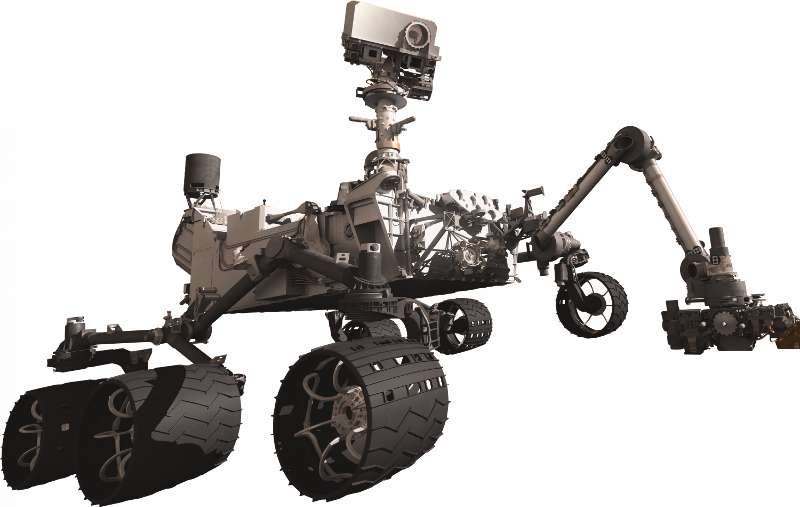
\includegraphics[height=\graphicsHeight]{sections/state-of-the-art/past-missions/images/rover-msl.png}
		\subcaption{MSL Curiosity}
		\label{fig:sub:past-mission-rovers-msl}
	\end{subfigure}
    \caption[Past and ongoing rover missions]
            {Past and ongoing rover missions.}
	\label{fig:past-mission-rovers}
\vspace{-2ex}
\end{figure}

\begin{comment}

\vspace{0.5cm}

\begin{figure}[h]
\captionsetup[subfigure]{justification=centering}
\vspace{-2ex}
	\centering
    %% setup sizes
    \setlength{\subfigureWidth}{0.32\textwidth}
    \setlength{\graphicsHeight}{30mm}
    %% kill hyper-link highlighting
    \hypersetup{hidelinks=true}%
    %% the figures
	\begin{subfigure}[t]{\subfigureWidth}
        \centering
		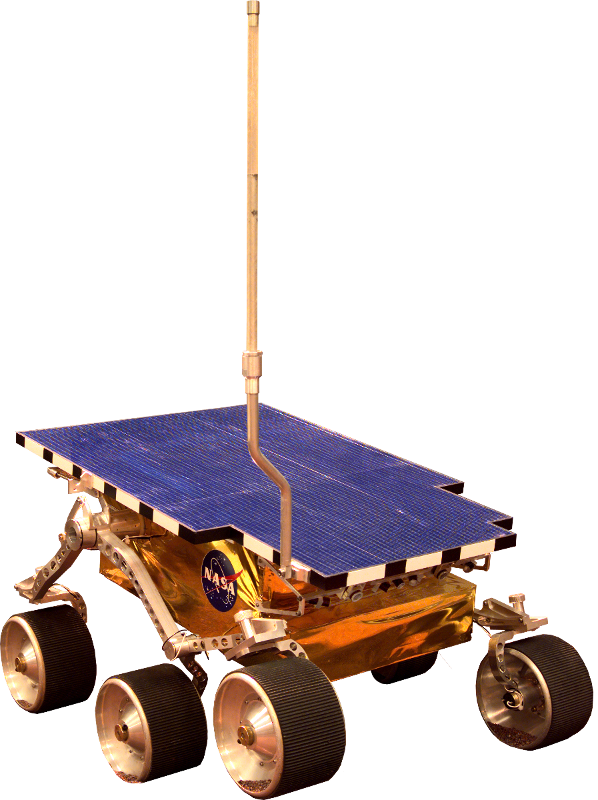
\includegraphics[height=\graphicsHeight]{sections/state-of-the-art/past-missions/images/rover-sojourner.png}
		\subcaption{Sojourner}
		\label{fig:sub:past-mission-rover-sojourner}
	\end{subfigure}\hfill
	\begin{subfigure}[t]{\subfigureWidth}
        \centering
		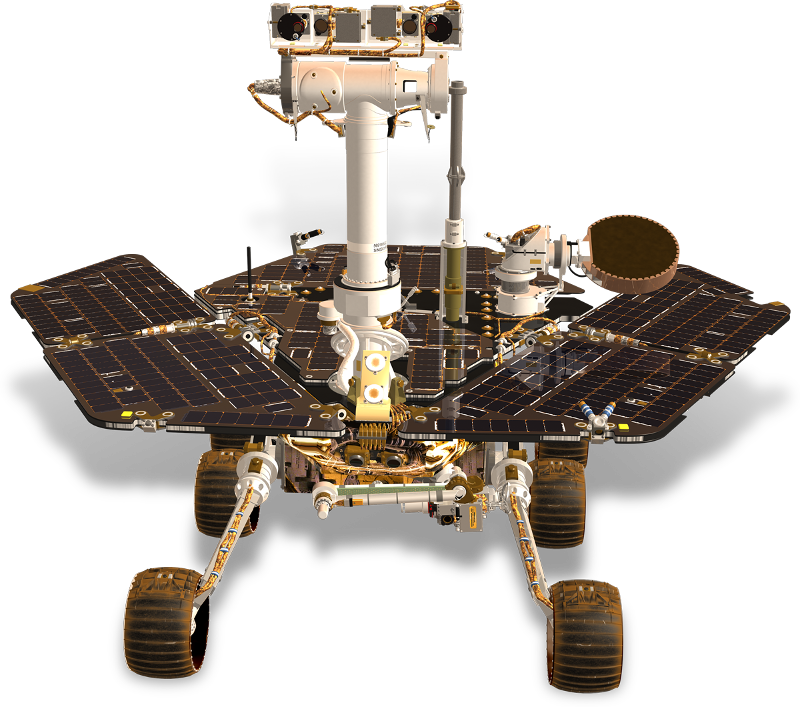
\includegraphics[height=\graphicsHeight]{sections/state-of-the-art/past-missions/images/rover-mer.png}
		\subcaption{MER Opportunity and Spirit}
		\label{fig:sub:past-mission-rovers-mer}
	\end{subfigure}\hfill
    \begin{subfigure}[t]{\subfigureWidth}
        \centering
		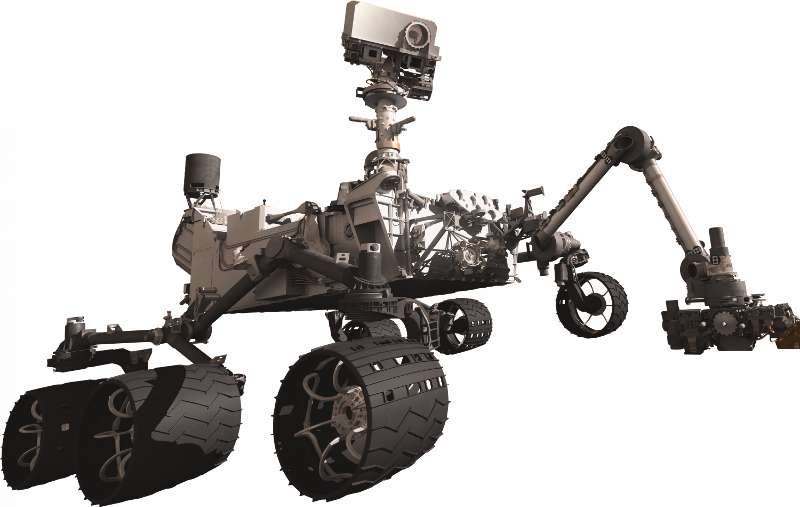
\includegraphics[height=\graphicsHeight]{sections/state-of-the-art/past-missions/images/rover-msl.png}
		\subcaption{MSL Curiosity}
		\label{fig:sub:past-mission-rovers-msl}
	\end{subfigure}
	\caption[Past and ongoing rover missions]
            {Past and ongoing rover missions.}
	\label{fig:past-mission-rovers}
\vspace{-2ex}
\end{figure}
\end{comment}

\subsubsection{Sojourner}
The Sojourner microrover was powered by a 0.22\si{\meter\squared}, $\SI{2}{\centi\meter}\times\SI{4}{\centi\meter}$, 5.5 mil thick \ac{GaAs}/\ac{Ge} solar panel. it provided around \SI{16.5}{\watt} of power at solar noon and the operating temperature was from \SI{-140}{\celsius} to +\SI{110}{\celsius}. Each of its three batteries were configured as 3 \ac{Li-SOCL2} D-size cells arranged in series and provided up to \SI{150}{\watt\hour}. The battery cell capacity was \SI{12}{\ampere\hour} at +\SI{25}{\celsius} and \SI{8}{\ampere\hour} at \SI{-20}{\celsius}. Operating voltage was 8‒11 \si{\volt} and mass was 1.24 \si{\kilo\gram}. The rover's power system allowed it to draw of up \SI{30}{\watt} of peak power with a peak solar panel power output of \SI{16}{\watt}. The rover's nominal propulsion power requirement is \SI{10}{\watt}. Further details on Sojourner's power subsystem can be found in \citepower{SojournerDescription} and \citepower{SojournerPowerSubsystem}.

\subsubsection{Opportunity and Spirit}
The twin rovers generated power from their triplejunction \ac{GaInP}/\ac{GaAs}/\ac{Ge} \acp{SA} with a solar cell coverage area of \SI{1.3}{\square\meter}. The \acp{SA} could generate almost \SI{900}{\watt\hour} of energy at \ac{BOL} on a clear day in absence of dust deposition \citepower{Badescu2009}. The rovers's propulsion power draw was approximately \SI{100}{\watt}. Two rechargeable \ac{Li-ion} NCP-8-1 \ac{NCO}-cell batteries weighing \SI{7.15}{\kilo\gram} were manufactured by Yardney and provided support to the \ac{SA} as well as enabled nighttime experiments \citepower{Badescu2009}. Each battery was configured in 8-cell \SI{10}{\ampere\hour} strings connected in parallel (8s2p). The nameplate capacity was \SI{8}{\ampere\hour} and the \ac{DOD} was designed to typically be 40‒50 \si{\percent} per Sol \citepower{Gulbinska2014}. Capacity voltage range was 16‒20 \si{\volt}, operating voltage range 24‒32.8 \si{\volt}, specific energy \SI{90}{\watt\hour/\kilo\gram}, and the operating temperature was from \SI{-20}{\celsius} to +\SI{30}{\celsius} \citepower{NASAEnergyStorage2017}. The rovers were heated by eight \acp{RHU}, each of which continuously generated \SI{1}{\watt} of thermal energy. The following are notable battery operational requirements taken from \citepower{Gulbinska2014}:

\begin{itemize}
  \item Maintaining the operating voltage of 24‒36 \si{\volt}.
  \item Providing sufficient energ for surface operations ($\geq$ \SI{283}{\watt\hour} per Sol at \SI{0}{\celsius}).
  \item Delivering sufficiently long cycle life ($\geq$ 270 cycles at \SI{50}{\percent} \ac{DOD} and/or 90 Sols operation).
  \item The battery should successfully charge and discharge between -20 and +\SI{30}{\celsius} throughout the length of the entire mission.
\end{itemize}

\subsubsection{Curiosity}
The Curiosity rover uses the \ac{MMRTG} power system. Is is designed to initially provide around \SI{2000}{\watt} of thermal power and \SI{110}{\watt} of electrical power in a deep space environment \citepower{MMRTG}. The electrical output is used to charge its two Yardney \ac{Li-ion} NCP-42-1 \ac{NCO}-cell batteries, which have a nameplate capacity rating of \SI{42}{\ampere\hour}. Curiosity's battery cells are arranged in an 8s2p configuration, capacity voltage range is 86‒92 \si{\volt}, operating voltage range 24‒32.8 \si{\volt}, mass \SI{26.5}{\kilo\gram}, specific energy \SI{104}{\watt\hour/\kilo\gram}, and the operating temperature is from \SI{-20}{\celsius} to +\SI{30}{\celsius} \citepower{NASAEnergyStorage2017}. The following are notable battery performance requirements taken from \citepower{Smart2009}:

\begin{itemize}
  \item Operation for more than 40 months after launch and a calendar life of $>$ 4 years.
  \item Provide 670 cycles of up to \SI{310}{\watt\hour} at 0‒\SI{30}{\celsius}, with a \SI{22}{\ampere} max capability to \SI{25}{\volt}.
  \item Provide 670 cycles of up to \SI{295}{\watt\hour} at -20 to +\SI{30}{\celsius}, with a \SI{10}{\ampere} max to \SI{25}{\volt}.
  \item Provide 670 cycles of up to \SI{555}{\watt\hour} at 0 to +\SI{30}{\celsius}, with a \SI{22}{\ampere}  max to \SI{25}{\volt} (only once per Martian Sol).
  \item Possess capability of meeting the performance requirements with an average battery temperature of +\SI{15}{\celsius} and an absolute maximum of +\SI{30}{\celsius} on the surface of Mars.
\end{itemize}


\clearpage
\section{Planned Missions}
\label{sec:StateOfTheArt:PlannedMissions}
Mars mission launch windows only occur once every 26 months, as showin in Figure \ref{fig:mars-distance-from-earth}. This section presents the power systems of Mars surface missions planned for the next window.

\begin{figure}[h]
  \captionsetup[subfigure]{justification=centering}
  \centering
  \hypersetup{linkcolor=captionTextColor}
  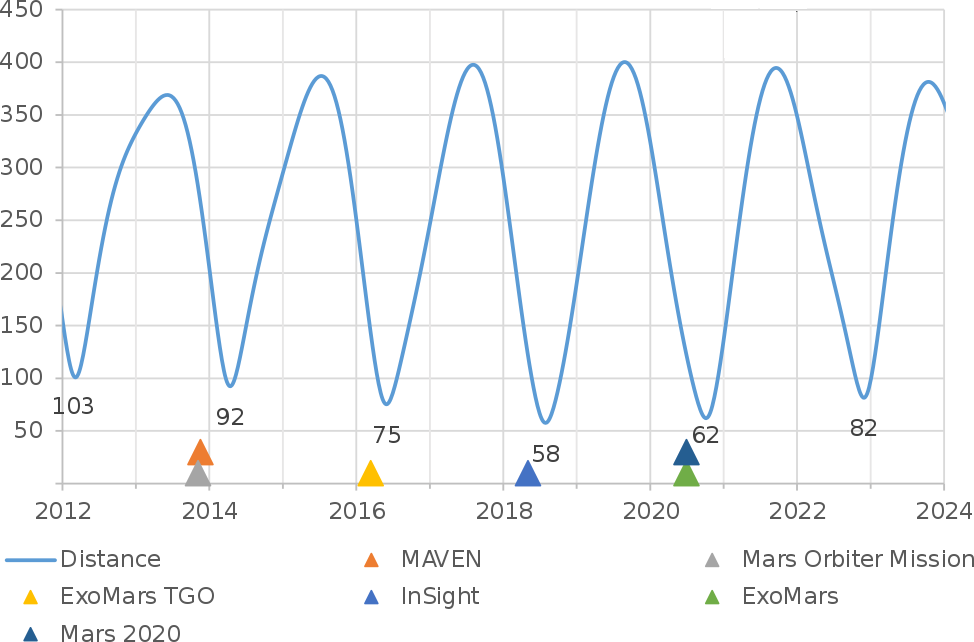
\includegraphics[width=0.5\linewidth]{sections/state-of-the-art/planned-missions/plots/mars-distance-from-earth.png}\\
  \caption[Spacecraft launches and Mars distance from Earth]
          {Spacecraft launches and Mars distance from Earth (Gm). Data source: HORIZONS System, JPL, NASA.}
  \label{fig:mars-distance-from-earth}
\end{figure}

At the time of writing this thesis, two rover missions are set to be launched during the next window: \ac{NASA}'s Mars 2020 rover, shown in Figure \ref{fig:sub:planned-mission-rover-mars2020}, and the \ac{ESA}/Roscosmos' ExoMars Rosalind Franklin rover, shown in Figure \ref{fig:sub:planned-mission-rover-exomars}.

\vspace{0.5cm}

\begin{figure}[h]
\captionsetup[subfigure]{justification=centering}
\vspace{-2ex}
	\centering
    %% setup sizes
    \setlength{\graphicsHeight}{50mm}
    %% kill hyper-link highlighting
    \hypersetup{hidelinks=true}%
    %% the figures
	\begin{subfigure}[t]{0.65\textwidth}
        \centering
		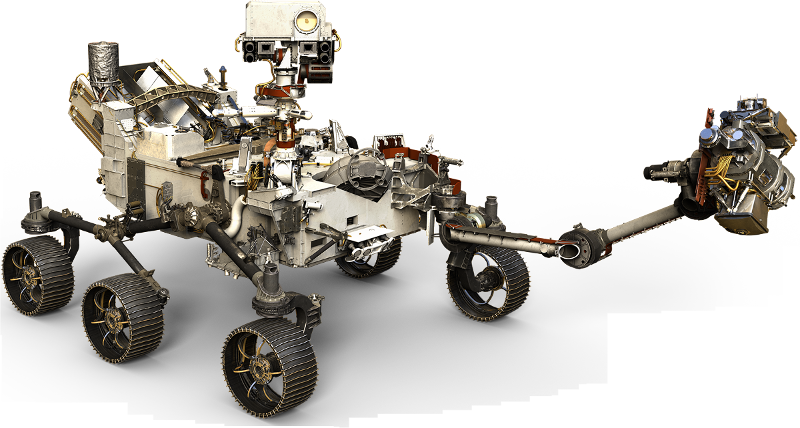
\includegraphics[height=\graphicsHeight]{sections/state-of-the-art/planned-missions/images/rover-mars2020.png}
		\subcaption{Mars 2020}
		\label{fig:sub:planned-mission-rover-mars2020}
	\end{subfigure}\hfill
	\begin{subfigure}[t]{0.35\textwidth}
        \centering
		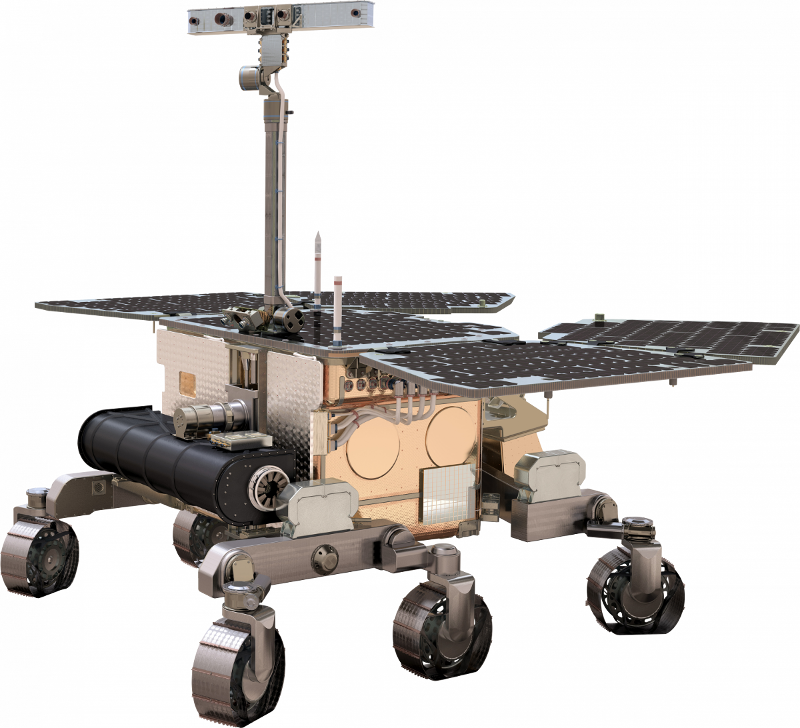
\includegraphics[height=\graphicsHeight]{sections/state-of-the-art/planned-missions/images/rover-exomars.png}
		\subcaption{Rosalind Franklin}
		\label{fig:sub:planned-mission-rover-exomars}
	\end{subfigure}
	\caption[Planned rover missions]
            {Planned rover missions. Mars 2020 is part of \ac{NASA}'s \ac{MEP}. Rosalind Franklin is part of the international ExoMars programme led by \ac{ESA} and Roscosmos}
	\label{fig:planned-mission-rovers}
\vspace{-2ex}
\end{figure}

\subsection{Mars 2020}
\label{sec:StateOfTheArt:PlannedMissions:Mars2020}

Mars 2020 is part of \ac{NASA}'s \ac{MEP}. Much of its design is based on heritage from the Curiosity mission. Its power system is identical to that of Curiosity in that it is equipped with a \ac{MMRTG} that will provide approximately \SI{110}{\watt} of electrical power at \ac{BOL}, declining by a few percent per year \citepower{Mars2020ElecticalPower}. Its two \ac{Li-ion} batteries are also identical to that of Curiosty and was previously elaborated on in Section \ref{sec:StateOfTheArt:PastAndOngoingMissions:Rovers}.

\subsection{Rosalind Franklin}
\label{sec:StateOfTheArt:PlannedMissions:RosalindFranklin}

Rosalind Franklin is part of the international ExoMars programme led by \ac{ESA} and Roscosmos. Its \ac{SA} is designed to generate up to \SI{1200}{\watt\hour} of energy \citepower{SaftPressRelease}. The \ac{SA} power output requirements are:

\begin{itemize}
    \item \ac{BOL}: $P_{max} > \SI{261}{\watt}$ under \SI{471}{Wm^{-2}}, \SI{-26}{\celsius}, and one string fail.
    \item \ac{EOL}: $P_{max} > \SI{131}{\watt}$ under \SI{358}{Wm^{-2}}, \SI{-52}{\celsius}, \SI{34}{\percent} dust coverage, and one string fail plus losses.
\end{itemize}

Test results detailed in \citepower{Riva2019} have measured \ac{SA} performances of $P_{max} = \SI{277}{\watt}$ for \ac{BOL} and $P_{max} = \SI{133.4}{\watt}$ for \ac{EOL}. The rover's battery cells are arranged in a 8s3p configuration and have an operational temperature range of \SI{-40}{\celsius} to +\SI{85}{\celsius} \citepower{EDN}. The rover is equipped with \acp{RHU} in order to maintain its internal temperature above \SI{-40}{\celsius}. The \ac{Li-ion} battery cells are manufactured by Saft and have the following specifications:

\begin{itemize}
    \item Nominal voltage: 3.65 \si{\volt}.
    \item Voltage range: 2.5‒\SI{4.2}{\volt}.
    \item Nameplate capacity: \SI{5.6}{\ampere\hour}.
    \item Nameplate energy:
    \begin{itemize}
        \item \ac{BOL}: \SI{1140}{\watt\hour}  under +\SI{50}{\celsius}, \SI{50}{\percent}. \ac{SOC}.
        \item End of cruise: \SI{980}{\watt\hour} under +\SI{40}{\celsius}, \SI{50}{\percent} \ac{SOC}.
        \item \ac{EOL}: \SI{790}{\watt\hour} under \SI{-20}{\celsius}, \SI{40}{\percent}. \ac{DOD}.
    \end{itemize}
\end{itemize}

The battery characterstics taken from \citepower{Amos2017} are as follow:

\begin{itemize}
    \item Operating voltage: 21‒\SI{29.4}{\volt}.
    \item Mass: $<$ \SI{10.5}{\kilo\gram}.
    \item Charge current:
    \begin{itemize}
        \item T $>$ \SI{0}{\celsius}: up to \SI{3}{\ampere}.
        \item T $<$ \SI{0}{\celsius}: up to \SI{5.2}{\ampere}.
    \end{itemize}
    \item Discharge current:  up to \SI{15}{\ampere}.
\end{itemize}


\clearpage
\section{Photovoltaics and Energy Storage}
\label{sec:StateOfTheArt:PhotovoltaicsAndEnergyStorage}
\subsection{Solar Cells}
At the time of writing this thesis, the InSight lander is the most recent solar powered mission currently operating on the Martian surface. On its first Sol, it generated a record breaking \SI{4.6}{\kilo\watt\hour} of energy. Its``UltraFlex'' \acp{SA} are manufactored by Orbital ATK.

\subsubsection{Triple Junction}
The ``UltraFlex'' \acp{SA} are made from from SolAero \ac{ZTJ} \ac{InGaP}/\ac{InGaAs}/\ac{Ge} space solar cells that boast a \SI{29.5}{\percent} \ac{BOL} efficiency at maximum power point for \ac{AM0} and \SI{135.3}{\milli\watt/\centi\meter^{2}} \citepower{SolAeroZTJDataSheet}. Similar solar cells with idential efficiencies are also available from other manufacturers such as Emcore \citepower{EmcoreZTJDataSheet}. \ac{TJ} \ac{GaAs} junction solar cells manufactured by AzureSpace advertise an average effeciency of \SI{29.5}{\percent} at \SI{1367}{\watt/\centi\meter^{2}} and \SI{29.8}{\percent} at \SI{1353}{\watt/\centi\meter^{2}} for \ac{AM0}, \SI{28}{\celsius} \citepower{AzureSpaceTJDataSheet}.

\subsubsection{Quadruple Junction}
\ac{QJ} solar cells of type \ac{AlInGaP}/\ac{AlInGaAs}/\ac{InGaAs}/\ac{Ge} on \ac{Ge} substrate manufactured by AzureSpace have an average efficiency of \SI{31.8}{\percent} at \ac{BOL} for \ac{AM0}, \SI{1367}{\watt/\centi\meter^{2}}, \SI{25}{\celsius} \citepower{AzureSpaceQJDataSheet}. \ac{QJ} solar cells with high theoretical efficiency of \SI{47.2}{\percent} have been proposed in \citepower{Hossain2016} as well as up to \SI{50}{\percent} efficiency with \ac{InGaP}/\ac{InGaAs}/\ac{InGaAsN}/\ac{Ge} in \citepower{Bestam2016}.

\subsubsection{Inverted Metamorphic Multi Junction}
Space-grade \ac{IMM} solar cells manufactured by SolAero have a typical \ac{BOL} efficiency of \SI{32}{\percent} at maximum power point for \ac{AM0}, \SI{135.3}{\milli\watt/\centi\meter^{2}}, and \SI{28}{\celsius} \citepower{SolAeroIMMDataSheet}. Series-connected \ac{5J} and \ac{6J} concentrator solar cell strategies have been proposed in \citepower{Geisz2017} as an extension to \ac{QJ} \ac{IMM} for a potential to exceed \SI{50}{\percent} efficiency.

\subsection{Battery Cells}
The battery cell presented in this section were selected from manufacturers that provided cells for InSight, Mars 2020, and Rosalind Franklin.

\subsubsection{Yardney EaglePicher}
The \ac{SOA} with Yardney EaglePicher are \ac{NCA} \ac{Li-ion} space battery cells with nominal capacity options of \SI{43}{\ampere\hour} or \SI{60}{\ampere\hour} at C/5 and \SI{20}{\celsius}. They share the same voltage range from 3 to \SI{4.1}{\volt} with a nominal voltage of \SI{3.6}{\volt}. The following specifications are taken from \citepower{EaglePicher43AhBatteryCell} and are specific to the \SI{43}{\ampere\hour} cells:

\begin{itemize}
    \item Energy density: \SI{378}{\watt\hour/l}.
    \item Specific energy: \SI{153}{\watt\hour/\kilo\gram}.
    \item Operating temperature: \SI{-20}{\celsius} to +\SI{60}{\celsius}.
    \item Charging method: constant \SI{21.5}{\ampere} (0.5C) current to \SI{4.1}{\volt}. and a constant voltage  \SI{4.1}{\volt} to 0.86 \si{\ampere} (C/50).
    \item Discharge rates with a maximum constant curent of \SI{200}{\ampere}.
\end{itemize}

The following specifications are from \citepower{EaglePicher60AhBatteryCell} and are specific to the \SI{60}{\ampere\hour} cells:

\begin{itemize}
    \item Energy density: \SI{393}{\watt\hour/l}.
    \item Specific energy: \SI{160}{\watt\hour/\kilo\gram}.
    \item Operating temperature: \SI{-20}{\celsius} to +\SI{40}{\celsius}.
    \item Charging method: constant \SI{12}{\ampere} (0.2C) current to \SI{4.1}{\volt} and a constant voltage \SI{4.1}{\volt} to \si{1.2}{\ampere} (C/50).
    \item Discharge rates with a maximum constant curent of \SI{250}{\ampere}.
\end{itemize}

\subsubsection{Saft}
Saft's prismatic MP and cylindrical VL rechargeable \ac{Li-ion} battery cells have the lowest temperature performance for charging, operating down to \SI{-50}{\celsius}. The following specifications are taken from \citepower{SaftSpaceBatteryCell}:

\begin{itemize}
  \item Nominal voltage: 3.6‒\SI{3.75}{\volt}.
  \item Energy density: up to \SI{385}{\watt\hour/l}.
  \item Specific energy: \SI{180}{\watt\hour/\kilo\gram}.
  \item Power range: up to \SI{1}{\kilo\watt/\kilo\gram}.
  \item Capacity range: 2.6‒\SI{7.0}{\ampere\hour}.
  \item Operating temperature: \SI{-20}{\celsius} to +\SI{60}{\celsius} for charge and \SI{-50}{\celsius} to +\SI{60}{\celsius} for discharge.
\end{itemize}


\section{Summary and Conclusion}
\label{sec:StateOfTheArt:SummaryAndConclusion}
Solar and battery cells are reviewed for past, ongoing, and planned Mars surface missions in order to appreciate technological limitations. From this analysis the \ac{IMM} solar cell is selected thus introducing an \ac{EOL} efficiency of \SI{22.5}{\percent} that must be considered during \ac{SA} sizing.
